%=============================================================================
%  CHAPTER 5 — REALIZATION OF THE MOBILE APPLICATION
%=============================================================================
\chapter{Realization of the Mobile Application}

\clearpage
\section*{Introduction}

The mobile application extends the reach of ForsaDrive by making the service available from any smartphone. Because carpooling is, by nature, something users organize on the move --- while leaving a class, waiting for a colleague, or standing at a louage station --- the mobile experience was treated as a first-class citizen and not as an afterthought. This chapter describes the technologies that were used to build it, the features that only make sense on a mobile device, and the main screens delivered at the end of the project. It closes with the testing strategy that was applied to the entire platform.


\section{Mobile Technologies}

\subsection{Choice of a Cross-Platform Framework}

Two main options were considered for the mobile application: developing natively for Android and iOS on the one hand, or using a cross-platform framework on the other. Native development would have doubled the effort without providing enough additional value for a ride-sharing use case, so a cross-platform framework was preferred. After evaluating the alternatives against the time budget of the internship and the team's experience, \textbf{Flutter} was selected.

Flutter is an open-source UI toolkit maintained by Google that allows a single Dart codebase to compile into genuinely native applications for Android, iOS, web, and desktop. Unlike JavaScript-based frameworks that bridge to native components at runtime, Flutter draws its own widgets using the Skia rendering engine, which gives it pixel-perfect consistency across platforms and excellent rendering performance. Its hot-reload feature also significantly accelerated the development cycle during the iterative sprints.

\begin{figure}[H]
    \centering
    \includegraphics[width=0.3\textwidth]{flutter_logo.png}
    \caption{Flutter logo}
    \label{fig:flutter_logo}
\end{figure}

\subsection{Supporting Libraries}

Several packages were added to the Flutter project to cover the specific needs of the application.

\begin{description}[noitemsep]
    \item[go\_router] Manages declarative navigation between screens, deep links, and the bottom tab bar.
    \item[provider] Implements the ChangeNotifier-based state management pattern, used for authentication state, locale, and ride data.
    \item[dio / http] Consumes the REST API exposed by the PHP backend, with the bearer token attached globally through an interceptor.
    \item[shared\_preferences] Persists the session token and the selected language locally on the device so that the user does not have to log in at every launch.
    \item[flutter\_map] Renders interactive OpenStreetMap tiles and draws the route polyline between the origin and the destination of a ride.
    \item[firebase\_messaging] Delivers push notifications for new bookings, confirmations, ride updates, and chat messages, even when the application is in the background.
    \item[flutter\_localizations] Provides the full internationalization infrastructure for French, English, and Arabic, including automatic RTL layout flipping for Arabic.
\end{description}

\section{Mobile-Specific Features}

Beyond mirroring the web experience, the mobile application takes advantage of features that only a phone can provide.

\subsection{Push Notifications}

Push notifications are delivered through Firebase Cloud Messaging. They inform the user of events that require attention: a new booking request for a driver, a booking confirmation or cancellation for a passenger, a ride departure, a new chat message, or an admin action on the account. Notifications are delivered even when the application is in the background, which matches the real usage patterns of the platform.

\subsection{In-App Chat}

The mobile application embeds a real-time messaging interface. Conversations are polled every three seconds to display new messages without requiring a persistent WebSocket connection. The interface shows date dividers, read receipts, and a typing indicator. Passengers and drivers can start a conversation directly from a booking notification without leaving the application.

\subsection{Interactive Map}

Each ride detail screen embeds a \texttt{FlutterMap} widget that geocodes the origin and destination city names using the Nominatim API and draws the driving route between them using the OSRM open routing service. Green and red markers indicate the pickup and drop-off points respectively.

\subsection{Multilingual Interface}

The application supports three languages --- French, English, and Arabic --- with a language picker accessible from the settings screen. Arabic triggers an automatic RTL layout flip through \texttt{GlobalWidgetsLocalizations}, so all padding, alignment, and navigation directions are mirrored without any manual override in the widget code.

\section{Presentation of the Mobile Interfaces}

The following screens illustrate the main paths inside the mobile application. Screens are shown in the order a typical passenger would go through them.

\subsection{Authentication}

The authentication screens cover login, registration, and student email OTP verification. The registration form includes a gender selector, a date-of-birth picker, and a real-time student domain detector that shows a green banner when the entered email belongs to a recognized university domain.

\begin{figure}[H]
    \centering
    \includegraphics[width=0.6\textwidth]{mobile_auth.png}
    \caption{Mobile authentication screens (login and registration)}
    \label{fig:mobile_auth}
\end{figure}

\subsection{Home and Search}

The home screen is centered on a search bar. Below it, three personalized sections are displayed: recommended rides based on the user's booking history (collaborative filtering), trending routes derived from recent bookings, and nearby rides matched to the user's governorate.

\begin{figure}[H]
    \centering
    \includegraphics[width=0.6\textwidth]{mobile_home.png}
    \caption{Home screen with personalized recommendations}
    \label{fig:mobile_home}
\end{figure}

\subsection{Ride Search and Filters}

The search results screen allows passengers to filter rides by price range, minimum driver rating, departure date, number of seats, and on-board amenities (air conditioning, Wi-Fi, music, accessibility). Each ride card displays a compatibility score badge showing how well the ride matches the passenger's profile and history.

\begin{figure}[H]
    \centering
    \includegraphics[width=0.6\textwidth]{mobile_search.png}
    \caption{Ride search results with filters and match score}
    \label{fig:mobile_search}
\end{figure}

\subsection{Trip Details and Booking}

After selecting a ride, the passenger reaches a detailed view that shows the route on an interactive map, the driver's profile and reliability score, and the price breakdown including the student discount when applicable. The booking is confirmed after the fifty-percent prepayment is deducted from the wallet.

\begin{figure}[H]
    \centering
    \includegraphics[width=0.9\textwidth]{mobile_trip_details.png}
    \caption{Trip details with map and booking confirmation}
    \label{fig:mobile_trip_details}
\end{figure}

\subsection{Driver Dashboard}

The driver dashboard is organized into two tabs. The overview tab shows active ride cards with departure and arrival action buttons. The analytics tab presents a reliability score gauge, a six-month revenue trend chart, a rating distribution bar chart, and smart improvement recommendations generated by the backend.

\begin{figure}[H]
    \centering
    \includegraphics[width=0.9\textwidth]{mobile_driver_dashboard.png}
    \caption{Driver dashboard with analytics and reliability score}
    \label{fig:mobile_driver_dashboard}
\end{figure}

\subsection{Wallet}

The wallet screen consolidates the financial activity of the user: current balance, pending amounts, and the history of operations. Drivers also see their earnings grouped by trip.

\begin{figure}[H]
    \centering
    \includegraphics[width=0.6\textwidth]{mobile_wallet.png}
    \caption{Wallet screen}
    \label{fig:mobile_wallet}
\end{figure}

\subsection{Social Feed}

The feed screen lets drivers post ride offers and passengers post travel requests. Posts can be liked, commented on, and used as a direct booking entry point through a quick-booking bottom sheet. Boosted posts appear at the top of the feed and are marked with a ``Boosted'' badge.

\begin{figure}[H]
    \centering
    \includegraphics[width=0.6\textwidth]{mobile_feed.png}
    \caption{Social feed with ride posts and quick booking}
    \label{fig:mobile_feed}
\end{figure}

\subsection{In-App Chat}

The chat screen lists the conversations linked to active trips. Each conversation opens on a messaging view with a bubble layout, date dividers, and read receipts. Drivers can also open a conversation directly from a booking notification.

\begin{figure}[H]
    \centering
    \includegraphics[width=0.6\textwidth]{mobile_chat.png}
    \caption{In-app chat screen}
    \label{fig:mobile_chat}
\end{figure}

\subsection{HelpDesk with AI Bot}

The HelpDesk screen opens a support conversation that is initially handled by a rule-based bot. The bot covers fourteen topic categories and responds instantly to common questions. When the bot cannot resolve the issue, it escalates the conversation to a human support agent and notifies the user.

\begin{figure}[H]
    \centering
    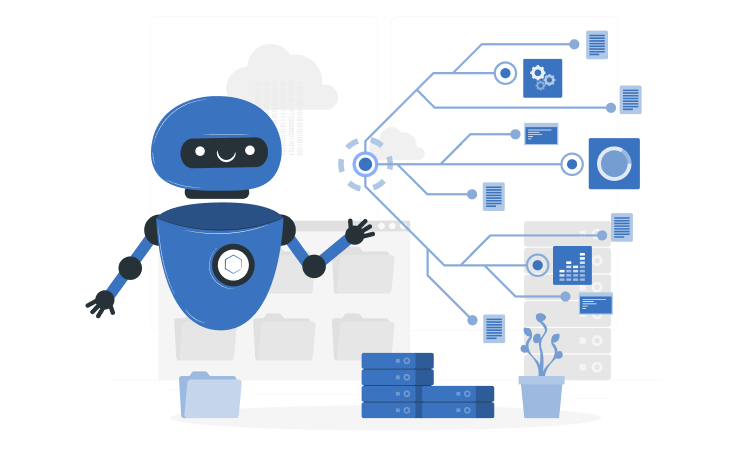
\includegraphics[width=0.6\textwidth]{aibot.png}
    \caption{HelpDesk screen with AI bot and escalation to human agent}
    \label{fig:mobile_helpdesk}
\end{figure}

\subsection{Profile and Settings}

The profile screen gathers the personal information, the verification status including the student badge, the vehicle list, and the language selector. A driver application card shows the status of any pending driver registration request.

\begin{figure}[H]
    \centering
    \includegraphics[width=0.6\textwidth]{mobile_profile.png}
    \caption{Profile and settings screen}
    \label{fig:mobile_profile}
\end{figure}

\section{Testing}

Testing was carried out continuously during the implementation phase, rather than left to a final stage.

\subsection{Unit Testing}

Unit tests were written for the most sensitive business rules of the backend: the computation of the total amount, the application of the student discount, the enforcement of the prepayment percentage, and the validation of user inputs. These tests catch regressions early and serve as a living documentation of the rules.

\subsection{Integration Testing}

Integration tests were performed through Postman collections that replay the main scenarios end to end: registration, login, trip creation, booking, payment, and rating. Each collection was executed after every significant change on the backend.

\subsection{Manual Testing}

Manual tests were conducted on the web application and on the mobile application, including cross-device testing on several Android phones. Feedback from members of the host organization also helped detect usability issues that automated tests cannot catch.

\subsection{Summary of Tests}

\begin{table}[H]
\centering
\caption{Summary of tested scenarios}
\begin{tabular}{|l|c|}
\hline
\textbf{Scenario}                             & \textbf{Result} \\
\hline
Registration and student email OTP verification & Passed \\
\hline
Login and token-based session                 & Passed \\
\hline
Driver application submission and approval    & Passed \\
\hline
Publishing, updating, and cancelling a trip   & Passed \\
\hline
Searching trips with filters and match score  & Passed \\
\hline
Booking with 50\% prepayment                  & Passed \\
\hline
Applying the student discount                 & Passed \\
\hline
Wallet top-up and history                     & Passed \\
\hline
Rating a completed trip                       & Passed \\
\hline
Real-time chat between two users              & Passed \\
\hline
Push notification delivery (FCM)              & Passed \\
\hline
Social feed post, like, comment, quick book   & Passed \\
\hline
Ride boosting with balance deduction          & Passed \\
\hline
Administrator moderation actions (7 tabs)     & Passed \\
\hline
Multilingual switching (FR / EN / AR + RTL)   & Passed \\
\hline
\end{tabular}
\end{table}

\section*{Conclusion}

This chapter closed the realization phase of ForsaDrive by presenting the mobile application and the testing strategy applied to the entire platform. The Flutter client reuses the PHP backend designed in the previous chapters and adds the features that a phone makes possible: push notifications, interactive maps, real-time chat, and a multilingual interface with automatic RTL support. Together with the web application, it delivers the complete ride-sharing experience originally targeted by the project.
